\documentclass[12pt, a4paper]{report}
\usepackage[utf8]{inputenc}
\usepackage[english, russian]{babel}

\usepackage{graphicx}
\usepackage{listings}
\usepackage{color}

\usepackage{amsmath}
\usepackage{pgfplots}
\usepackage{url}
\usepackage{flowchart}
\usepackage{tikz}
\DeclareGraphicsExtensions{.pdf,.png,.jpg,.svg}
\usetikzlibrary{shapes, arrows}

\usepackage{pgfplotstable}

\renewcommand\contentsname{Содержание}

\usepackage{geometry}
\geometry{left=3cm}
\geometry{right=1cm}
\geometry{top=2cm}
\geometry{bottom=2cm}

\lstset{ %
language=C++,                 % выбор языка для подсветки (здесь это С)
basicstyle=\small\sffamily, % размер и начертание шрифта для подсветки кода
numbers=left,               % где поставить нумерацию строк (слева\справа)
numberstyle=\tiny,           % размер шрифта для номеров строк
stepnumber=1,                   % размер шага между двумя номерами строк
numbersep=-5pt,                % как далеко отстоят номера строк от         подсвечиваемого кода
backgroundcolor=\color{white}, % цвет фона подсветки - используем         \usepackage{color}
showspaces=false,            % показывать или нет пробелы специальными     отступами
showstringspaces=false,      % показывать или нет пробелы в строках
showtabs=false,             % показывать или нет табуляцию в строках
frame=single,              % рисовать рамку вокруг кода
tabsize=2,                 % размер табуляции по умолчанию равен 2 пробелам
captionpos=t,              % позиция заголовка вверху [t] или внизу [b] 
breaklines=true,           % автоматически переносить строки (да\нет)
breakatwhitespace=false, % переносить строки только если есть пробел
escapeinside={\%*}{*)},   % если нужно добавить комментарии в коде
keywordstyle=\color{blue}\ttfamily,
stringstyle=\color{red}\ttfamily,
commentstyle=\color{green}\ttfamily,
morecomment=[l][\color{magenta}]{\#},
columns=fullflexible }

\usepackage{titlesec}
\titleformat{\chapter}[hang]{\LARGE\bfseries}{\thechapter{.} }{0pt}{\LARGE\bfseries}
\titleformat*{\section}{\Large\bfseries}
\titleformat*{\subsection}{\large\bfseries}

\begin{document}

    \begin{titlepage}

        \begin{center}
            \Large
            {\sl Государственное образовательное учреждение высшего профессионального образования\\
            {\bf«Московский государственный технический университет имени Н.Э. Баумана»\\
				(МГТУ им. Н.Э. Баумана)}}
				\noindent\rule{\textwidth}{2pt}
            \vspace{3cm}

			{\scshape\LARGE Лабораторная работа №2 \par}
			\vspace{0.5cm}	
			{\scshape\LARGE по курсу «Анализ алгоритмов» \par}
			\vspace{1.5cm}
			{\huge\bfseries Умножение матриц \par}
			\vspace{2cm}
			\Large Выполнил: Сорокин А.П., гр. ИУ7-52Б\\
			\vspace{0.5cm}
			{\Large Преподаватели: Волкова Л.Л., Строганов Ю.В.}
		
			\vfill
			\Large \textit {Москва, 2019 г.}
            
        \end{center}

    \end{titlepage}
	
	\tableofcontents

	\chapter*{Введение}
	\addcontentsline{toc}{chapter}{Введение}
	
	\hspace{1cm}В огромном количестве областей научной и технической сферы деятельности человека при различных математических расчетах используют такую операцию как умножение матриц. Это довольно трудоемкий процесс даже при небольших размерах матриц, так как требуется большое количество операций умножения и сложения различных чисел. По этой причине человек озадачен проблемой оптимизации умножения матриц и ускорения процесса вычисления.\\
	Таким образом, эффективное умножение матриц по времени и затратам ресурсов является актуальной проблемой для науки и техники.

    \chapter{Аналитическая часть}
	\section{Задачи}
	Цель лабораторной работы - изучение трех алгоритмов умножения матриц: классического, алгоритма Винограда и его оптимизации.\\
	Для того чтобы добиться этой цели, были поставлены следующие задачи:
	\begin{itemize}
		\item изучить и реализовать классический алгоритм умножения матриц и алгоритм Винограда;
		\item оптимизировать работу алгоритма Винограда;
		\item выполнить сравнительный анализ трудоёмкостей алгоритмов;
		\item сравнить эффективность алгоритмов по времени и памяти.
	\end{itemize}

	\section{Описание алгоритмов}
	
	\subsection{Классический алгоритм умножения}
	Матрицей называют математический объект, эквивалентный двумерному массиву. Матрица является таблицей, на пересечении строк и столбцов находятся элементы матрицы. Количество строк и столбцов является размерностью матрицы.\\
	Пусть даны две прямоугольные матрицы A и B размерности $m \times n$, $n \times q$
	соответственно:\\
	$$A =  \begin{bmatrix} 
	a_{11}& a_{12} &\ldots & a_{1n}\\ 
	a_{21}& a_{22} &\ldots & a_{2n}\\ 
	\vdots& \vdots &\ddots & \vdots\\ 
	a_{m1}& a_{m2} &\ldots & a_{mn} 
	\end{bmatrix} $$\\	
	
	$$B = \begin{bmatrix} 
	b_{11}& b_{12} &\ldots & b_{1q}\\ 
	b_{21}& b_{22} &\ldots & b_{2q}\\ 
	\vdots& \vdots &\ddots & \vdots\\ 
	b_{n1}& b_{n2} &\ldots & b_{nq} 
	\end{bmatrix} $$\\
	
	Тогда произведением матриц A и B называется матрица C размерностью  $m \times q$ 
	\begin{equation}
	\label{matrix-mult}
	C = \begin{bmatrix} 
	c_{11} & c_{12} & \cdots & c_{1q} \\
	c_{21} & c_{22} & \cdots & c_{2q} \\ 
	\vdots & \vdots & \ddots & \vdots \\ 
	c_{m1} & c_{m2} & \cdots & c_{mq}	
	\end{bmatrix}, ~\cite{CompAlg}
	\end{equation}
	в которой:
	$$c_{ij} = \sum_{k=1}^n a_{ik}b_{kj} \;\;\; \left(\overline{i = 1 \ldots m};\;\overline{j = 1 \ldots q} \right).$$

	\subsection{Алгоритм Винограда}
	Исходя из равенства \ref{matrix-mult}, видно, что каждый элемент в нем представляет собой скалярное произведение соответствующих строки и столбца исходных матриц. Такое умножение допускает предварительную обработку, позволяющую часть работы выполнить заранее. ~\cite{Winograd}\\
	Рассмотрим два вектора U и V:
	
	\begin{equation}
	\label{u-def}
	U = A_{i} = (u_{1}, u_{2}, \ldots, u_{n}),
	\end{equation}
	где $U = A_{i}$ -- i-ая строка матрицы A,\\
	$u_{k} = a_{ik}, \overline{k = 1 \ldots n}$ -- элемент i-ой строки k-ого столбца матрицы A.\\
	
	\begin{equation}
	\label{v-def}
	V = B_{j} = (v_{1}, v_{2}, \ldots, v_{n}),
	\end{equation}
	где $V = B_{j}$ -- j-ый столбец матрицы B,\\
	$v_{k} = b_{kj}, \overline{k = 1 \ldots n}$ -- элемент k-ой строки j-ого столбца матрицы B.\\
	
	По определению их скалярное произведение равно:\\
	\begin{equation}
	\label{uv-def}
	U \cdot V = u_{1}v_{1} + u_{2}v_{2} + u_{3}v_{3} + u_{4}v_{4}.
	\end{equation}
	Равенство \ref{uv-def} можно переписать в виде:\\
	\begin{equation}
	\label{uv}
	U \cdot V = (u_{1} + v_{2})(u_{2} + v_{1}) + (u_{3} + v_{4})(u_{4} + v_{3}) - u_{1}u_{2} - u_{3}u_{4} - v_{1}v_{2} - v_{3}v_{4}.
	\end{equation}
	В равенстве \ref{uv-def} насчитывается 4 операции умножения и 3 операции сложения, в равенстве \ref{uv} насчитывается 6 операций умножения и 9 операций сложения. Однако выражение $- u_{1}u_{2} - u_{3}u_{4}$ используются повторно при умножении i-ой строки матрицы A на каждый из столбцов матрицы B, а выражение $- v_{1}v_{2} - v_{3}v_{4}$ - при умножении j-ого столбца матрицы B на строки матрицы A. Таким образом, данные выражения можно вычислить предварительно для каждых строк и столбцов матриц для сокращения повторных вычислений. В результате повторно будут выполняться лишь 2 операции умножения и 7 операций сложения (2 операции нужны для добавления предварительно посчитанных произведений).
	
	\subsection{Оптимизированный алгоритм Винограда}
	Для оптимизации алгоритма Винограда могут использоваться такие стратегии, как:
	\begin{itemize}
		\item предварительные вычисления повторяющихся одинаковых действий;
		\item использование более быстрых операций при вычислении (такие, как смещение битов вместо умножения или деления на 2);
		\item уменьшения количества повторных проверок;
		\item использование аналогичных конструкций, уменьшающих трудоёмкость операций (к примеру, замена сложения с 1 на инкремент).
	\end{itemize}
	Ниже представлен список личностей, проводивших оптимизацию алгоритма:
	\begin{itemize}
		\item в 2010 Эндрю Стотерс усовершенствовал алгоритм до $O(n^{2.374})$;
		\item в 2011 году Вирджиния Уильямс усовершенствовала алгоритм до $O(n^{2.3728642})$;
		\item в 2014 году Франсуа Ле Галль упростил метод Уильямса и получил новую улучшенную оценку $O(n^{2.3728639})$.
	\end{itemize}
	
	\subsection{Модель вычислений}
	В рамках данной работы используется следующая модель вычислений:
	\begin{itemize}
		\item операции, имеющие трудоемкость 1: $<$, $>$, $=$, $<=$, $=>$, $==$, $!=$,$+$, $-$, $\ast$, /, $+$=, $-$=, $\ast$=, $/$=, [ ];
		\item оператор условного перехода имеет трудоёмкость, равную трудоёмкости операторов тела условия;
		\item оператор цикла for имеет трудоемкость:
		\begin{equation}
		\label{for_cost}
		F_{for} = F_{init} + F_{check} + N \ast (F_{body} + F_{inc} + F_{check}),
		\end{equation}
		где $F_{init}$ -- трудоёмкость инициализации, $F_{check}$ -- трудоёмкость проверки условия, $F_{inc}$ -- трудоёмкость инкремента аргумента, $F_{body}$ -- трудоёмкость операций в теле цикла, $N$ -- число повторений. ~\cite{AlgAnalysis}
	\end{itemize} 
	

	\chapter{Конструкторская часть}
	
	\section{Схемы алгоритмов}
	На рисунках \ref{pic:clasic}, \ref{pic:vin}, \ref{pic:optvin} представлены схемы алгоритмов трёх алгоритмов умножения матриц.
	\begin{figure}[ht!]
		\centering
		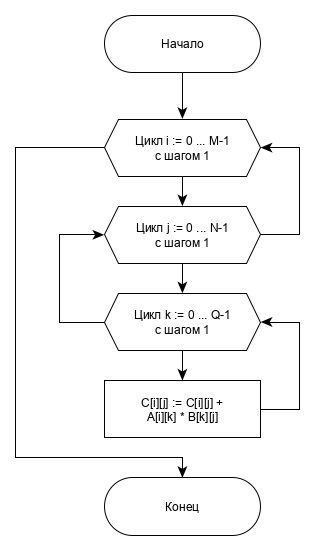
\includegraphics[scale=0.8]{classic.jpg}
		\caption{Классический алгоритм}
		\label{pic:clasic}
	\end{figure}
	\newpage
	\begin{figure}[ht!]
		\centering
		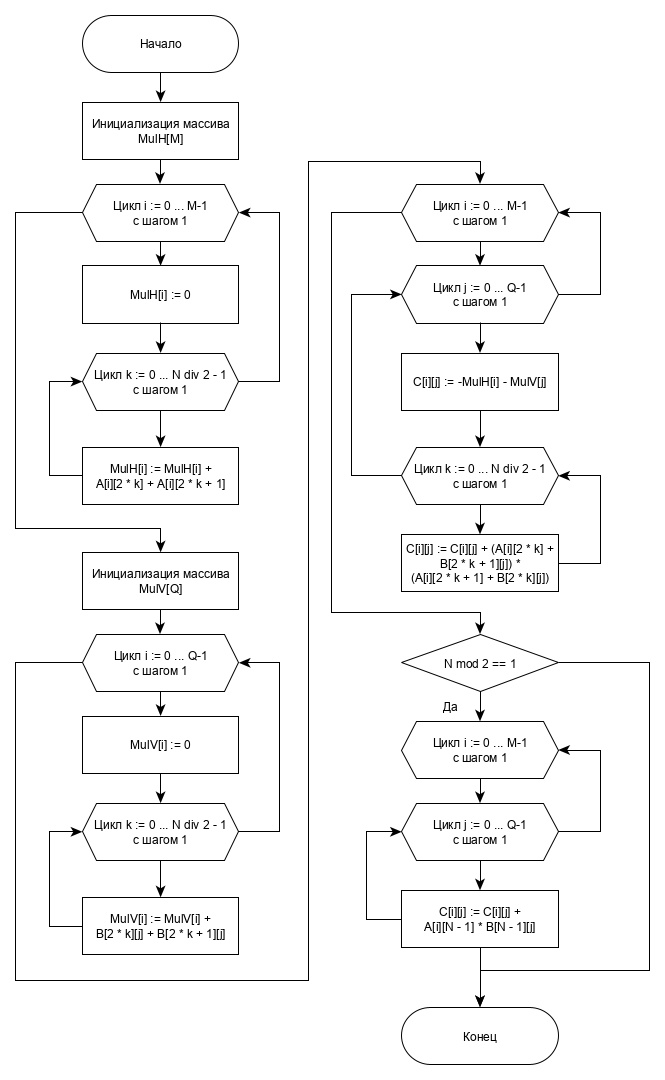
\includegraphics[scale=0.6]{vin.jpg}
		\caption{Алгоритм Винограда}
		\label{pic:vin}
	\end{figure}
	\newpage
	\begin{figure}[ht!]
		\centering
		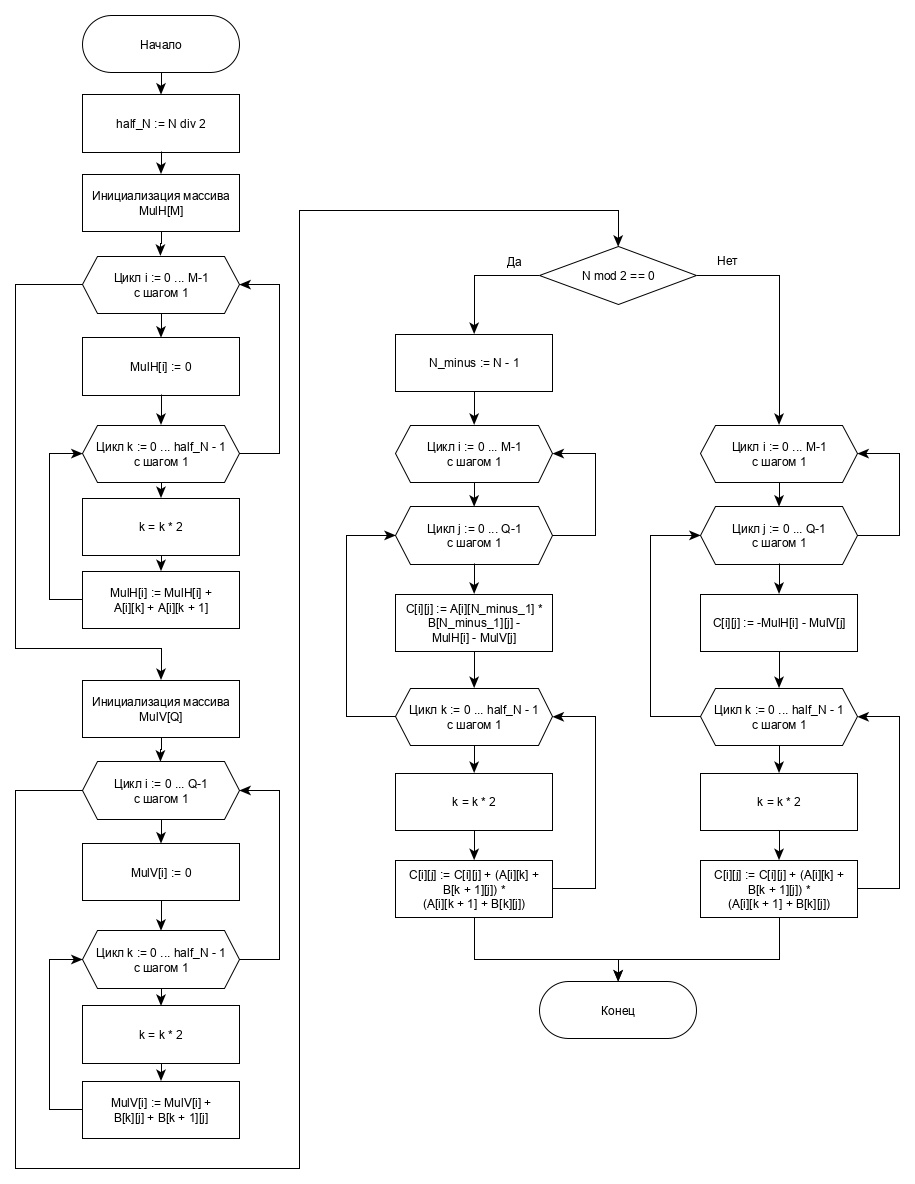
\includegraphics[scale=0.55]{vin_opt.jpg}
		\caption{Оптимизированный алгоритм Винограда}
		\label{pic:optvin}
	\end{figure}

	\newpage

	\section{Оценка трудоёмкости}
	Пусть даны две матрицы $A$ и $B$ размерностью $M\times N$ и размерностью $N \times Q$ соответственно. Рассмотрим трудоемкость трёх алгоритмов умножения матриц.
	
	\subsection{Классический алгоритм}
	\begin{equation}
	\label{complex_classic}
	f_{classic} = 13MNQ + 4MQ + 4M + 1
	\end{equation}
	
	\subsection{Алгоритм Винограда}
	Трудоёмкости составных частей алгоритма:
	\begin{itemize}
		\item цикл создания вектора MulH: $f_{I} = \frac{15}{2}MN + 4M + 2$;
		\item цикл создания вектора MulV:  $f_{II} = \frac{15}{2}NQ + 4Q + 2$;
		\item основной цикл: $f_{III} = 13MNQ + 4MQ + 4M + 2$;
		\item условный переход при чётном $N$: $f_{IV} = 2$;
		\item условный переход и цикл при нечётном $N$: $f_{IV} = 17MQ + 4M + 4$.
	\end{itemize}
	Общая трудоемкость алгоритма:
	\begin{itemize}
		\item при чётном $N$:
		\begin{equation}
		\label{complex_vin_even}
		f_{vin} = f_{I} + f_{II} + f_{III} + f_{IV} = 13MNQ + \frac{15}{2}MN + \frac{15}{2}NQ + 4MQ + 8M + 4Q + 8
		\end{equation}
		\item при нечётном $N$:
		\begin{equation}
		\label{complex_vin_odd}
		f_{vin} = f_{I} + f_{II} + f_{III} + f_{IV} = 13MNQ + \frac{15}{2}MN + \frac{15}{2}NQ + 21MQ + 12M + 4Q + 10
		\end{equation}
	\end{itemize}
	
	\subsection{Оптимизированный алгоритм Винограда}
	Трудоёмкости составных частей алгоритма:
	\begin{itemize}
		\item цикл создания вектора MulH: $f_{I} = \frac{11}{2}MN + 4M + 2$;
		\item цикл создания вектора MulV:  $f_{II} = \frac{11}{2}NQ + 4Q + 2$;
		\item основной цикл при чётном $N$: $f_{III} = 10MNQ + 17MQ + 4M + 6$;
		\item основной цикл при нечётном $N$: $f_{III} = 10MNQ + 10NQ + 4M + 2$.
	\end{itemize}
	Общая трудоемкость алгоритма:
	\begin{itemize}
		\item при чётном $N$:
		\begin{equation}
		\label{complex_vin_even}
		f_{opt} = f_{I} + f_{II} + f_{III} = 10MNQ + \frac{11}{2}MN + \frac{11}{2}NQ + 17MQ + 8M + 4Q + 10
		\end{equation}
		\item при нечётном $N$:
		\begin{equation}
		\label{complex_vin_odd}
		f_{opt} = f_{I} + f_{II} + f_{III} = 10MNQ + \frac{11}{2}MN + \frac{11}{2}NQ + 10NQ + 8M + 4Q + 6
		\end{equation}
	\end{itemize}

	\section{Список оптимизаций алгоритма Винограда}
	Алгоритм Винограда был оптимизирован с помощью следующих модификаций:
	\begin{enumerate}
		\item Замена конструкций вида a = a + b (трудоёмкость = 2) на a += b (трудоёмкость = 1).
		\item Вычисление повторно используемых величин выполняется предварительно ($N / 2$, $N - 1$, $2 * k$).
		\item Цикл вычислений для нечётных элементов включён в основной цикл, добавив дополнительные операции. Данная модификация исключает повторные проверки на нечётность $N$.
 	\end{enumerate}

	\section{Замер используемой памяти}
	Пусть даны две матрицы $A$ и $B$ размерностью $M\times N$ и размерностью $N \times Q$ соответственно и для хранения целого числа требуется 4 байта памяти.\\
	В каждом из алгоритмов требуется хранить исходные матрицы $A$ и $B$ и матрицу результата умножения $C$, которая имеет размеры $M \times Q$. Таким образом, под хранение матриц требуется $4 \cdot (MN + NQ + MQ)$ байт памяти.\\
	Для алгоритма Винограда и его оптимизированного варианта требуется также хранить два дополнительных вектора $MulH$ и $MulV$. Их размеры $M$ и $Q$ соответственно, следовательно требуется дополнительно $4 \cdot (M + Q)$ байт памяти. В итоге для алгоритмов Винограда требуется $4 \cdot (MN + NQ + MQ + M + Q)$ байт памяти. Таким образом, при больших размерах матриц (больше 100) алгоритмы Винограда будут значительно проигрывать по памяти классическому алгоритму.\\
	
	\chapter{Технологическая часть}
	\section{Требования к программному обеспечению}
	На вход подаются размеры двух матриц. Матрицы генерируются случайным образом и выводятся на экран. На выход программа выдаёт три матрицы, которые являются результатами работы трёх различных алгоритмов умножения.
	\section{Средства реализации}
	Для реализации программы был использован язык C++ ~\cite{CPP}. Для замера процессорного времени была использована функция rdtsc() из библиотеки stdrin.h.
	\section{Реализации алгоритмов}
	В листингах \ref{code-classic}, \ref{code-vin}, \ref{code-opt} представлены коды реализации алгоритмов умножения матриц.
	\begin{lstlisting}[label=code-classic,caption=Классический алгоритм]
	void multiply_classic(int **A, int **B, int **C, unsigned M, unsigned N, unsigned Q)
	{
		for (unsigned i = 0; i < M; i++)
			for (unsigned j = 0; j < Q; j++)
			{
				C[i][j] = 0;
				for (unsigned k = 0; k < N; k++)
					C[i][j] += A[i][k] * B[k][j];
			}
	}
	\end{lstlisting}

	\begin{lstlisting}[label=code-vin,caption=Алгоритм Винограда]
	void multiply_vinograd(int **A, int **B, int **C, unsigned M, unsigned N, unsigned Q)
	{
		int *MulH = new int[M];
		for (unsigned i = 0; i < M; i++)
		{
			MulH[i] = 0;
			for (unsigned k = 0; k < N / 2; k++)
				MulH[i] = MulH[i] + A[i][2 * k] * A[i][2 * k + 1];
		}
		
		int *MulV = new int[Q];
		for (unsigned i = 0; i < Q; i++)
		{
			MulV[i] = 0;
			for (unsigned k = 0; k < N / 2; k++)
				MulV[i] = MulV[i] + B[2 * k][i] * B[2 * k + 1][i];
		}
		
		for (unsigned i = 0; i < M; i++)
			for (unsigned j = 0; j < Q; j++)
			{
				C[i][j] = -MulH[i] - MulV[j];
				for (unsigned k = 0; k < N / 2; k++)
					C[i][j] = C[i][j] + (A[i][2 * k] + B[2 * k + 1][j]) *
								(A[i][2 * k + 1] + B[2 * k][j]);
			
			}
		
		if (N % 2 == 1)
			for (unsigned i = 0; i < M; i++)
				for (unsigned j = 0; j < Q; j++)
					C[i][j] = C[i][j] + A[i][N - 1] * B[N - 1][j];
		
		delete [] MulH;
		delete [] MulV;
	}
	\end{lstlisting}

	\begin{lstlisting}[label=code-opt,caption=Оптимизированный алгоритм Винограда]
	void multiply_vinograd_opt(int **A, int **B, int **C, unsigned M, unsigned N, unsigned Q)
	{
		int *MulH = new int[M];
		for (unsigned i = 0; i < M; i++)
		{
			MulH[i] = 0;
			for (unsigned k = 0; k < N; k <<= 1)
				MulH[i] += A[i][k] * A[i][k + 1];
		}
		
		int *MulV = new int[Q];
		for (unsigned i = 0; i < Q; i++)
		{
			MulV[i] = 0;
			for (unsigned k = 0; k < N; k << = 1)
				MulV[i] += B[k][i] * B[k + 1][i];
			}
		}
		
		if (N % 2)
		{
			unsigned N_minus_1 = N - 1;
			for (unsigned i = 0; i < M; i++)
				for (unsigned j = 0; j < Q; j++)
				{
					C[i][j] = A[i][N_minus_1] * B[N_minus_1][j] - MulH[i] - MulV[j];
					for (unsigned k = 0; k < N; k <<= 1)
						C[i][j] += (A[i][k] + B[k + 1][j]) * (A[i][k + 1] + B[k][j]);
				}
		}
		else
		{
			for (unsigned i = 0; i < M; i++)
				for (unsigned j = 0; j < Q; j++)
				{
					C[i][j] = -MulH[i] - MulV[j];
					for (unsigned k = 0; k < N; k <<= 1)
						C[i][j] += (A[i][k] + B[k + 1][j]) * (A[i][k + 1] + B[k][j]);
				}
		}
		
		delete [] MulH;
		delete [] MulV;
	}
	\end{lstlisting}

	\newpage

	\section{Тесты}
	Для проверки корректности работы были подготовлены функциональные тесты, представленные в таблице \ref{unit-tests}. Входные данные удовлетворяют условиям, необходимым для умножения матриц, так как проверка на соответствие их размеров возложена на другую функцию.

	\begin{table}[ht!]
		\caption{Функциональные тесты}
		\label{unit-tests}
		\begin{center}
			\begin{tabular}{|c|c|c|}
			\hline
			\bf{Матрица 1} & \bf{Матрица 2} & \bf{Ожидание}\\\hline
			
			$\begin{bmatrix}5\end{bmatrix}$ &
			$\begin{bmatrix}-8\end{bmatrix}$ &
			$\begin{bmatrix}-40\end{bmatrix}$\\\hline
			
			$\begin{bmatrix}2 & 1 & 1\end{bmatrix}$ &
			$\begin{bmatrix}1\\-1\\5\end{bmatrix}$ &
			$\begin{bmatrix}6\end{bmatrix}$\\\hline
			
			$\begin{bmatrix}5 & 1\\0 & -1\end{bmatrix}$ &
			$\begin{bmatrix}3 & -5\\10 & 0\end{bmatrix}$ &
			$\begin{bmatrix}-10 & 25\\-10 & 0\end{bmatrix}$\\\hline
			
			$\begin{bmatrix}1 & 2 & 0\\3 & 0 & -1\end{bmatrix}$ &
			$\begin{bmatrix}1 & 2\\3 & 0\\0 & -2\end{bmatrix}$ &
			$\begin{bmatrix}7 & 2\\3 & 8\end{bmatrix}$\\\hline
			
			$\begin{bmatrix}1 & 1 & -1\\5 & -3 & -4\end{bmatrix}$ &
			$\begin{bmatrix}0 & 0\\0 & 0\\0 & 0\end{bmatrix}$ &
			$\begin{bmatrix}0 & 0\\0 & 0\end{bmatrix}$\\\hline
			
			$\begin{bmatrix}1 & 0\\0 & 1\end{bmatrix}$ &
			$\begin{bmatrix}1 & 3\\-2 & 1\end{bmatrix}$ &
			$\begin{bmatrix}1 & 3\\-2 & 1\end{bmatrix}$\\\hline

			\end{tabular}
		\end{center}
	\end{table}

	В результате проверки реализации всех алгоритмов умножения прошли все поставленные функциональные тесты.

	\chapter{Экспериментальная часть}
	\section{Примеры работы}
	На рисунке \ref{pic:example} представлен пример работы программы, демонстрирующий корректную работу алгоритмов.
	\begin{figure}[ht!]
		\centering
		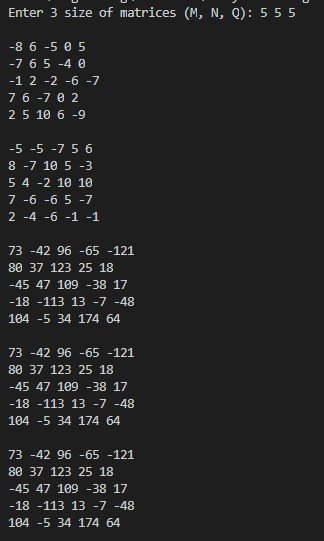
\includegraphics[scale=0.8]{example.jpg}
		\caption{Пример работы программы}
		\label{pic:example}
	\end{figure}
	
	\section{Сравнение работы алгоритмов при чётных размерах матрицы}
	Для сравнения времени работы алгоритмов умножения матриц были использованы квадратные матрицы размером от 100 до 1000 с шагом 100. Эксперимент для более точного результата повторялся 100 раз. Итоговый результат рассчитывался как средний из полученных результатов. Результаты измерений показаны в таблице \ref{table-even} и на рисунке \ref{graph-even}.\\
	\begin{table}[ht!]
		\caption{Время работы алгоритмов при чётных размерах матриц в тактах процессора}
		\label{table-even}
		\begin{center}
			\pgfplotstabletypeset[
			col sep=semicolon,
			string type,
			columns/Size/.style={column name=Размер матриц, column type={|c}},
			columns/Classic/.style={column name=Классический, column type={|c}},
			columns/Vinograd/.style={column name=Алг-м Виногада, column type={|c}},
			columns/VinOptimized/.style={column name=Оптимиз. алг-м Винограда, column type={|c|}},
			every head row/.style={before row=\hline,after row=\hline},
			every last row/.style={after row=\hline},
			]{EvenTime.csv}
		\end{center}
	\end{table}
	
	\begin{figure}[ht!]
		\begin{tikzpicture}
		\begin{axis}
			[%title = График времени работы алгоритмов при чётных размерах матриц,
			table/col sep = semicolon,
			xlabel={Размер матриц},
			ylabel={Время в тиках},
			ymin = 0,
			legend pos=outer north east,
			ymajorgrids=true,
			grid style=dashed]
			\addplot[color=red, mark=*] table[x={Size}, y={Classic}] {EvenTime.csv};
			\addplot[color=blue, mark=*] table[x={Size}, y={Vinograd}] {EvenTime.csv};
			\addplot[color=green, mark=*] table[x={Size}, y={VinOptimized}] {EvenTime.csv};
			\legend{Классический алг-м, Алг-м Винограда, Оптимиз. алг-м Винограда}
		\end{axis}
		\end{tikzpicture}
		\caption{График времени работы алгоритмов при чётных размерах матриц}
		\label{graph-even}
	\end{figure}

	\newpage
	
	Из результатов экспериментов можно сделать вывод о том, что алгоритм Винограда выигрывает классический алгоритм умножения матриц в среднем на 18\%. Оптимизированный алгоритм работает незначительно, но быстрее обычного алгоритма Винограда.
	
	\section{Сравнение работы алгоритмов при нечётных размерах матрицы}
	Для сравнения времени работы алгоритмов умножения матриц были использованы квадратные матрицы размером от 101 до 1001 с шагом 100. Эксперимент для более точного результата повторялся 100 раз. Итоговый результат рассчитывался как средний из полученных результатов. Результаты измерений показаны в таблице \ref{table-odd} и на рисунке \ref{graph-odd}.\\
	
	\begin{table}[ht!]
		\caption{Время работы алгоритмов при нечётных размерах матриц в тактах процессора}
		\label{table-odd}
		\begin{center}
			\pgfplotstabletypeset[
			col sep=semicolon,
			string type,
			columns/Size/.style={column name=Размер матриц, column type={|c}},
			columns/Classic/.style={column name=Классический, column type={|c}},
			columns/Vinograd/.style={column name=Алг-м Виногада, column type={|c}},
			columns/VinOptimized/.style={column name=Оптимиз. алг-м Винограда, column type={|c|}},
			every head row/.style={before row=\hline,after row=\hline},
			every last row/.style={after row=\hline},
			]{OddTime.csv}
		\end{center}
	\end{table}

	\begin{figure}[ht!]
		\begin{tikzpicture}
		\begin{axis}
		[%title = График времени работы алгоритмов при нечётных размерах матриц,
		table/col sep = semicolon,
		xlabel={Размер матриц},
		ylabel={Время в тиках},
		ymin = 0,
		legend pos=outer north east,
		ymajorgrids=true,
		grid style=dashed]
		\addplot[color=red, mark=*] table[x={Size}, y={Classic}] {OddTime.csv};
		\addplot[color=blue, mark=*] table[x={Size}, y={Vinograd}] {OddTime.csv};
		\addplot[color=green, mark=*] table[x={Size}, y={VinOptimized}] {OddTime.csv};
		\legend{Классический алг-м, Алг-м Винограда, Оптимиз. алг-м Винограда}
		\end{axis}
		\end{tikzpicture}
		\caption{График времени работы алгоритмов при нечётных размерах матриц}
		\label{graph-odd}
	\end{figure}

	\newpage
	
 	Для случая с нечётными размерами матриц можно сделать те же выводы, что и для случая с чётными. При этом можно заметить, что классический алгоритм в среднем работает за то же время, что и при чётных размерах, в то время как алгоритм Винограда и его оптимизация работают дольше за счёт дополнительных операций при нечётном случае. Однако по-прежнему классический алгоритм проигрывает по времени на те же величины.

	\chapter*{Заключение}
	\addcontentsline{toc}{chapter}{Заключение}
	В ходе лабораторной работе были изучены и реализованы три алгоритма умножения матриц: классический алгоритм, алгоритм Винограда и его оптимизированный вариант. Сравнительный анализ алгоритмов показал, что алгоритмы Винограда, введя дополнительные векторы и увеличив тем самым расход памяти, добились уменьшения времени выполнения умножения за счёт уменьшения трудоёмких операций: неоптимизированный и оптимизированный варианты работают на 18-20\% быстрее классического алгоритма.
	
	\newpage
	
	\begin{thebibliography}{}
	\bibitem{CompAlg} Бахвалов, Н.С. Численные методы / Н.С. Бахвалов, Н.П. Жидков, Г.М. Кобельков – М.: Наука, 1987.
	\bibitem{Winograd} Jelfimova L. A new fast systolic array for modified Winograd algorithm // Proc. Sevens Int. Workshop on Parallel Processing by Cellular Automata and Array, PARCELLA-96 (Berlin, Germany, Sept. 1996). — Berlin: Akad. Verlag. — 1996.
	\bibitem{AlgAnalysis} Кормен, Т. Алгоритмы: построение и анализ / Т. Кормен, Ч. Лейзерсон, Р.М. Ривест: – МЦНТО, 1999.
	\bibitem{CPP} https://cppreference.com/ [Электронный ресурс]
	\end{thebibliography}
	\addcontentsline{toc}{chapter}{Литература}

\end{document}
